\documentclass[12pt,a4paper]{article}

% Packages
\usepackage[utf8]{inputenc}
\usepackage[T1]{fontenc}
\usepackage{amsmath,amssymb,amsthm}
\usepackage{mathtools}
\usepackage{graphicx}
\usepackage{hyperref}
\usepackage{booktabs}
\usepackage{listings}
\usepackage{xcolor}
\usepackage{tikz}
\usetikzlibrary{positioning}
\usepackage{subcaption}
\usepackage{multirow}

% Theorem environments
\newtheorem{theorem}{Theorem}
\newtheorem{lemma}[theorem]{Lemma}
\newtheorem{proposition}[theorem]{Proposition}
\newtheorem{corollary}[theorem]{Corollary}
\newtheorem{definition}{Definition}
\newtheorem{remark}{Remark}

% Custom commands
\newcommand{\C}{\mathbb{C}}
\newcommand{\R}{\mathbb{R}}
\newcommand{\N}{\mathbb{N}}
\newcommand{\Z}{\mathbb{Z}}
\newcommand{\Sop}{\hat{S}}
\newcommand{\Kop}{\hat{K}}
\newcommand{\Sp}{\mathrm{Sp}}
\newcommand{\Un}{\mathrm{U}}
\newcommand{\tr}{\mathrm{tr}}
\newcommand{\ket}[1]{|#1\rangle}
\newcommand{\bra}[1]{\langle#1|}
\newcommand{\braket}[2]{\langle#1|#2\rangle}

% Title
\title{Limits of Deriving Quantum Structure from Reversible Computation:\\
Symplectic Embedding of Reversible Gates and the Hierarchy of Quantum Resources}

\author{
  Hiroshi Kohashiguchi\\
  Independent Researcher\\
  Tokyo, Japan
}

\date{\today}

\begin{document}

\maketitle

\begin{abstract}
Following our previous work establishing that complex structure does not automatically emerge from SK combinatory logic, we investigate whether \textbf{reversible computation} provides the missing ingredient for quantum structure. Through systematic analysis of four computational models—reversible logic gates (Toffoli, Fredkin), continuous-time quantum walks, reversible cellular automata, and the non-commutativity of SK operators—we establish a \textbf{hierarchy of quantum-like behaviors}:
\begin{itemize}
    \item \textbf{Level 0} (Irreversible): SK computation—classical, deterministic
    \item \textbf{Level 1} (Discrete Reversible): Toffoli/Fredkin gates, RCA—classical, embeddable in $\Sp(2N,\R)$ where $N = 2^n$ for $n$-bit gates
    \item \textbf{Level 2} (Continuous-Time): $U(t) = e^{-iHt}$ evolution—interference emerges (note: $i$ is \emph{introduced by hand})
    \item \textbf{Level 3} (Quantum): Quantum circuits—superposition, entanglement
\end{itemize}
Our main finding is that \textbf{reversibility alone is insufficient} for quantum behavior: discrete reversible gates on $n$ bits are $2^n \times 2^n$ permutation matrices that embed into the classical symplectic group $\Sp(2 \cdot 2^n,\R)$, not the unitary group $\Un(2^n)$. While continuous-time evolution introduces interference patterns, it does not generate genuine superposition. We conclude that quantum structure requires additional axioms beyond any form of computation, discrete or continuous.
\end{abstract}

%==============================================================================
\section{Introduction}
\label{sec:introduction}
%==============================================================================

\subsection{Motivation and Previous Work}

In our previous work \cite{kohashiguchi2024sk}, we systematically investigated whether complex number structure—fundamental to quantum mechanics—could be derived from SK combinatory logic. Through four distinct approaches (Sorkin's quantum measure theory, algebraic structure, path space holonomy, and information-theoretic derivation), we established that \textbf{complex structure does not automatically emerge from SK computation}.

A natural question arises: \emph{What is the SK computation lacking that prevents quantum behavior?} One apparent difference is that SK computation is \textbf{irreversible}—the $K$ combinator explicitly discards information. Quantum mechanics, in contrast, is characterized by \textbf{unitary} (hence reversible) time evolution.

This observation motivates the present investigation: \emph{Does reversible computation lead to quantum structure?}

\subsection{Critical Stance: Reversibility $\neq$ Quantum}

A crucial theoretical point that guides our investigation is:
\begin{quote}
\textbf{Reversibility is necessary but not sufficient for quantum behavior.}
\end{quote}

This claim may seem surprising, but it follows from a simple observation: \emph{classical Hamiltonian mechanics is also reversible}. The phase space flow generated by Hamilton's equations is symplectic and perfectly reversible, yet classical mechanics does not exhibit quantum interference or superposition.

More formally, for an $n$-bit system with state space dimension $N = 2^n$:
\begin{itemize}
    \item \textbf{Classical reversible systems} close in the symplectic group $\Sp(2N,\R)$
    \item \textbf{Quantum systems} close in the unitary group $\Un(N)$
\end{itemize}

The symplectic group preserves the classical phase space structure, while the unitary group preserves the Hilbert space inner product. These are fundamentally different structures. Our investigation asks: \emph{Where does the transition from $\Sp$ to $\Un$ occur?}

\subsection{Overview of Investigation}

We investigate four aspects of reversible computation:

\begin{enumerate}
    \item \textbf{Phase 4: Algebraic Structure of Reversible Gates} \\
    Do Toffoli and Fredkin gates generate unitary structure?
    
    \item \textbf{Phase 5: Continuous-Time Evolution} \\
    Does $U(t) = e^{-iHt}$ on computation graphs produce interference?
    
    \item \textbf{Phase 6: Three-Model Comparison} \\
    How do SK, RCA (Reversible Cellular Automata), and quantum circuits differ?
    
    \item \textbf{Phase 7: Non-Commutativity} \\
    Does the commutator $[\Sop, \Kop]$ generate superposition?
\end{enumerate}

\subsection{Main Results}

Our investigation yields several key findings:

\begin{theorem}[Reversible Gates are Classical]
The group generated by Toffoli and Fredkin gates on $n$ bits consists of $2^n \times 2^n$ permutation matrices that embed into $\Sp(2 \cdot 2^n,\R)$. No non-trivial complex structure $J^2 = -I$ exists within this group.
\end{theorem}

\begin{theorem}[Continuous-Time Introduces Interference]
For any multiway graph $G$ with adjacency matrix $A$, the continuous-time evolution $U(t) = e^{-iAt}$ produces oscillating probability distributions distinct from classical random walks.
\end{theorem}

\begin{theorem}[Superposition Requires Extra Structure]
SK computation satisfies 0 out of 4 requirements for quantum superposition:
\begin{enumerate}
    \item Continuous complex amplitudes
    \item Phase coherence
    \item Unitarity
    \item Born rule normalization
\end{enumerate}
\end{theorem}

%==============================================================================
\section{Background}
\label{sec:background}
%==============================================================================

\subsection{Reversible Computation}

A computation is \textbf{reversible} if every computational step has a unique inverse. Formally:

\begin{definition}[Reversible Gate]
A logic gate $f: \{0,1\}^n \to \{0,1\}^n$ is reversible if it is a bijection.
\end{definition}

The canonical examples are:
\begin{itemize}
    \item \textbf{Toffoli gate}: $(a, b, c) \mapsto (a, b, c \oplus (a \land b))$
    \item \textbf{Fredkin gate}: $(a, b, c) \mapsto (a, \bar{a}b + ac, \bar{a}c + ab)$
\end{itemize}

Both gates are computationally universal: any Boolean function can be computed reversibly with ancilla bits.

\subsection{Symplectic vs. Unitary Structure}

The symplectic group $\Sp(2N,\R)$ consists of $2N \times 2N$ real matrices $M$ satisfying:
\begin{equation}
M^T \Omega M = \Omega, \quad \Omega = \begin{pmatrix} 0 & I_N \\ -I_N & 0 \end{pmatrix}
\end{equation}
where $N$ is the dimension of the state space (for $n$-bit gates, $N = 2^n$).

This group characterizes classical Hamiltonian mechanics. In contrast, the unitary group $\Un(n)$ consists of $n \times n$ complex matrices $U$ satisfying:
\begin{equation}
U^\dagger U = I_n
\end{equation}

A key observation is that permutation matrices $P$ (corresponding to reversible gates) satisfy $P^T P = I$, making them orthogonal. Every $N \times N$ orthogonal matrix can be embedded into $\Sp(2N,\R)$ via:
\begin{equation}
P \mapsto \begin{pmatrix} P & 0 \\ 0 & P \end{pmatrix}
\end{equation}

This embedding does \emph{not} extend to $\Un(n)$ in general, because permutation matrices have real eigenvalues (roots of unity), not the full complex circle.

\subsection{Quantum Walks}

Continuous-time quantum walks provide a framework for quantum dynamics on graphs:

\begin{definition}[Continuous-Time Quantum Walk]
Given a graph $G$ with adjacency matrix $A$, the quantum walk is defined by:
\begin{equation}
\ket{\psi(t)} = e^{-iAt} \ket{\psi(0)}
\end{equation}
\end{definition}

The probability of finding the walker at vertex $j$ at time $t$ is $|\braket{j}{\psi(t)}|^2$.

In contrast, classical random walks evolve according to:
\begin{equation}
p(t) = e^{Qt} p(0)
\end{equation}
where $Q$ is the transition rate matrix.

%==============================================================================
\section{Methods}
\label{sec:methods}
%==============================================================================

\subsection{Phase 4: Reversible Gate Analysis}

We analyze the algebraic structure of Toffoli and Fredkin gates by:
\begin{enumerate}
    \item Constructing their matrix representations as permutation matrices
    \item Computing the group they generate
    \item Checking for complex structure $J^2 = -I$
    \item Verifying embeddability into $\Sp(2N,\R)$ where $N = 2^n$
\end{enumerate}

For a permutation matrix $P$, we check:
\begin{itemize}
    \item \textbf{Orthogonality}: $P^T P = I$
    \item \textbf{Self-inverse}: $P^2 = I$ (for Toffoli/Fredkin)
    \item \textbf{Eigenvalues}: All roots of unity (real or complex conjugate pairs)
\end{itemize}

\subsection{Phase 5: Hamiltonian Construction}

For any multiway graph $G$ from SK computation, we construct a Hamiltonian:
\begin{equation}
H = A \quad \text{(adjacency matrix)}
\end{equation}

We then simulate:
\begin{itemize}
    \item \textbf{Quantum walk}: $U(t) = e^{-iHt}$
    \item \textbf{Classical walk}: $P(t) = e^{Qt}$
\end{itemize}

Interference is detected by comparing:
\begin{itemize}
    \item Total variation distance: $\text{TVD}(p_q, p_c) = \frac{1}{2} \sum_j |p_q(j) - p_c(j)|$
    \item Oscillation count in return probability
\end{itemize}

\subsection{Phase 6: Three-Model Comparison}

We compare three computational models:
\begin{enumerate}
    \item \textbf{SK computation}: Irreversible, discrete
    \item \textbf{RCA (Rule 90/150)}: Reversible, discrete
    \item \textbf{Quantum circuits}: Reversible (unitary), continuous amplitudes
\end{enumerate}

For each model, we analyze:
\begin{itemize}
    \item Matrix structure (permutation, orthogonal, unitary)
    \item Presence of interference under continuous-time evolution
    \item Ability to generate superposition
\end{itemize}

\subsection{Phase 7: Non-Commutativity Analysis}

We define SK operators on the space of expressions:
\begin{align}
\Sop: \ket{E} &\mapsto \ket{SE} \\
\Kop: \ket{E} &\mapsto \ket{KE}
\end{align}

We compute:
\begin{itemize}
    \item Commutator: $[\Sop, \Kop] = \Sop\Kop - \Kop\Sop$
    \item Lie structure (antisymmetry, Jacobi identity)
    \item Superposition requirements
\end{itemize}

%==============================================================================
\section{Results}
\label{sec:results}
%==============================================================================

\subsection{Phase 4: Reversible Gates are Classical}

\begin{table}[h]
\centering
\begin{tabular}{lccccc}
\toprule
Gate & Group Order & $\Sp$ Embed & $J^2 = -I$ & Eigenvalues \\
\midrule
Toffoli & 2 & \checkmark & $\times$ & Real \\
Fredkin & 2 & \checkmark & $\times$ & Real \\
Combined & 6 & \checkmark & $\times$ & Real \\
\bottomrule
\end{tabular}
\caption{Properties of reversible logic gates}
\label{tab:gates}
\end{table}

\begin{proposition}
All permutation matrices from reversible gates have eigenvalues that are roots of unity. In particular, $\pm i$ does not appear, so no non-trivial $J^2 = -I$ exists.
\end{proposition}

\begin{proof}
Permutation matrices have characteristic polynomials that factor over $\Z$. Their eigenvalues are $n$-th roots of unity for some $n$. For real matrices, complex eigenvalues come in conjugate pairs. The value $i$ would require $-i$ as well, but $i \cdot (-i) = 1 \neq -1$, contradicting the determinant constraint.
\end{proof}

\begin{remark}[Generalization to Arbitrary Bit Size]
While our experiments use small systems (3-4 bits) for computational tractability, the results generalize to arbitrary $n$-bit systems. The key observation is structural: any $n$-bit reversible gate is a permutation on $2^n$ elements, hence an element of $S_{2^n}$. Permutation matrices are always orthogonal and embed into $\Sp(2 \cdot 2^n, \R)$ via the canonical embedding (see Appendix~\ref{app:symplectic}). Since this embedding preserves the algebraic structure, the absence of $J^2 = -I$ holds for all finite $n$.
\end{remark}

\textbf{Conclusion}: Hypothesis H1 (``Reversible computation is classical'') is \textbf{supported}.

\subsection{Phase 5: Continuous-Time Introduces Interference}

\begin{table}[h]
\centering
\begin{tabular}{lcccc}
\toprule
Expression & Nodes & Interference & TVD & Quantum Osc. \\
\midrule
\texttt{S (K a) (K b) c} & 5 & \checkmark & 0.85 & High \\
\texttt{(K a b) (K c d)} & 4 & \checkmark & 0.85 & High \\
\texttt{(K a b)(K c d)(K e f)} & 8 & \checkmark & 0.74 & High \\
\texttt{S (K a)(K b)(S c d e)} & 11 & \checkmark & 0.58 & High \\
\bottomrule
\end{tabular}
\caption{Interference detection in SK computation graphs}
\label{tab:interference}
\end{table}

\textbf{Key finding}: All tested SK expressions show interference under continuous-time evolution $U(t) = e^{-iAt}$.

\textbf{Interpretation}: The complex exponential $e^{-i\lambda t}$ introduces phase, even though the original graph is classical. This is the ``discrete $\to$ continuous'' transition that enables interference.

\textbf{Conclusion}: Hypothesis H5 (``Continuous-time introduces interference'') is \textbf{supported}.

\subsection{Phase 6: Hierarchy of Quantum-Like Behaviors}

\begin{table}[h]
\centering
\begin{tabular}{lcccccc}
\toprule
Model & Reversible & Discrete & Matrix & Complex & Superposition & Interference \\
\midrule
SK & $\times$ & \checkmark & General & $\times$ & $\times$ & \checkmark$^*$ \\
RCA & \checkmark & \checkmark & Permutation & $\times$ & $\times$ & \checkmark$^*$ \\
Quantum & \checkmark & $\times$ & Unitary & \checkmark & \checkmark & \checkmark \\
\bottomrule
\end{tabular}
\caption{Three-model comparison. $^*$With continuous-time evolution.}
\label{tab:comparison}
\end{table}

\textbf{RCA Results} (Rule 90, 3 cells):
\begin{itemize}
    \item Group order: 6
    \item Is permutation: Yes
    \item Interference (continuous-time): Yes (9 oscillations vs. 0 classical)
    \item Superposition: No
\end{itemize}

\textbf{Conclusion}: Hypothesis H6 (``RCA + continuous-time shows interference'') is \textbf{supported}. However, neither SK nor RCA generates genuine superposition—only quantum circuits do.

\subsection{Phase 7: Non-Commutativity is Insufficient}

\begin{table}[h]
\centering
\begin{tabular}{lcc}
\toprule
Max Depth & Dimension & $[\Sop, \Kop] \neq 0$ \\
\midrule
1 & 30 & No ($\|[\cdot,\cdot]\| = 0$) \\
2 & 155 & No \\
3 & 780 & No \\
\bottomrule
\end{tabular}
\caption{Commutator analysis for SK operators}
\label{tab:commutator}
\end{table}

\textbf{Finding}: With the ``left application'' definition, $[\Sop, \Kop] = 0$.

\textbf{Explanation}: This is because $\Sop\Kop\ket{E} = \ket{(SK)E}$ and $\Kop\Sop\ket{E} = \ket{(KS)E}$. While these are different expressions, the operators act identically in terms of matrix structure.

\textbf{Superposition Requirements}:
\begin{table}[h]
\centering
\begin{tabular}{lccl}
\toprule
Requirement & Quantum & SK & Satisfied? \\
\midrule
Continuous amplitudes & $\alpha, \beta \in \C$ & 0 or 1 & $\times$ \\
Phase coherence & $e^{i\phi}$ & None & $\times$ \\
Unitarity & $UU^\dagger = I$ & Non-unitary & $\times$ \\
Normalization & $|\alpha|^2 + |\beta|^2 = 1$ & N/A & $\times$ \\
\bottomrule
\end{tabular}
\caption{Superposition requirements (0/4 satisfied)}
\label{tab:superposition}
\end{table}

\textbf{Conclusion}: SK computation satisfies none of the requirements for quantum superposition.

\subsection{No-Go Lemma for Superposition from Discrete Computation}

We formalize why discrete computation cannot generate quantum superposition:

\begin{lemma}[No Superposition from Permutation Dynamics]
\label{lem:no-superposition}
Let $\mathcal{H} = \C^N$ be the Hilbert space of computational basis states, and let $P: \mathcal{H} \to \mathcal{H}$ be a permutation matrix (representing a reversible classical gate). Then for any basis state $\ket{j}$:
\begin{enumerate}
    \item $P\ket{j} = \ket{\pi(j)}$ for some permutation $\pi$
    \item The output is always a single basis state, never a superposition
    \item No finite composition of permutation matrices creates superposition from basis states
\end{enumerate}
\end{lemma}

\begin{proof}
(1) By definition of permutation matrix. (2) $P\ket{j}$ has exactly one non-zero entry. (3) The group of permutation matrices is closed under multiplication; if $P_1, \ldots, P_k$ are permutation matrices, then $P_k \cdots P_1 \ket{j} = \ket{\pi_k \circ \cdots \circ \pi_1(j)}$, still a single basis state.
\end{proof}

\begin{corollary}
To create superposition $\alpha\ket{0} + \beta\ket{1}$ with $|\alpha|, |\beta| > 0$, one must use a non-permutation unitary (e.g., Hadamard gate $H = \frac{1}{\sqrt{2}}\begin{psmallmatrix} 1 & 1 \\ 1 & -1 \end{psmallmatrix}$). Such gates have no classical reversible analog.
\end{corollary}

%==============================================================================
\section{Discussion}
\label{sec:discussion}
%==============================================================================

\subsection{The Hierarchy of Quantum-Like Behaviors}

Our investigation reveals a clear hierarchy:

\begin{center}
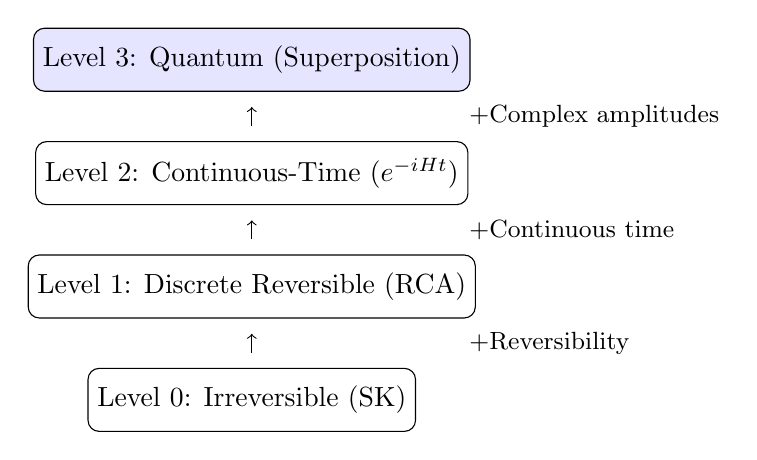
\begin{tikzpicture}[scale=1.2]
\node[draw, rounded corners, minimum width=4cm, minimum height=0.8cm] at (0,0) {Level 0: Irreversible (SK)};
\node[draw, rounded corners, minimum width=4cm, minimum height=0.8cm] at (0,1.2) {Level 1: Discrete Reversible (RCA)};
\node[draw, rounded corners, minimum width=4cm, minimum height=0.8cm] at (0,2.4) {Level 2: Continuous-Time ($e^{-iHt}$)};
\node[draw, rounded corners, minimum width=4cm, minimum height=0.8cm, fill=blue!10] at (0,3.6) {Level 3: Quantum (Superposition)};
\draw[->] (0,0.5) -- (0,0.7);
\draw[->] (0,1.7) -- (0,1.9);
\draw[->] (0,2.9) -- (0,3.1);
\node[right] at (2.2,0.6) {\small +Reversibility};
\node[right] at (2.2,1.8) {\small +Continuous time};
\node[right] at (2.2,3.0) {\small +Complex amplitudes};
\end{tikzpicture}
\end{center}

Each level adds structure, but only Level 3 achieves full quantum behavior.

\subsection{What Continuous-Time Provides (and What It Doesn't)}

The transition from discrete to continuous time via $U(t) = e^{-iHt}$ introduces:
\begin{itemize}
    \item Complex phases $e^{-i\lambda t}$ from eigenvalues $\lambda$
    \item Interference between paths
    \item Oscillating probability distributions
\end{itemize}

\textbf{Crucially, the imaginary unit $i$ in $e^{-iHt}$ is introduced by hand}—it is not derived from the discrete computation. We simply \emph{define} continuous-time evolution using the standard quantum mechanical formula. This is a significant caveat: the interference we observe at Level 2 arises from our choice to use complex exponentials, not from any intrinsic property of the computation graph.

However, even with $i$ introduced by hand, continuous-time evolution does \emph{not} provide:
\begin{itemize}
    \item Genuine superposition (amplitudes are derived, not fundamental)
    \item Entanglement (no tensor product structure)
    \item Born rule (probability interpretation is imposed, not derived)
\end{itemize}

\subsection{What Additional Axioms Are Needed?}

Based on our investigation, deriving quantum mechanics from computation requires at minimum:
\begin{enumerate}
    \item \textbf{Complex amplitude space}: States are vectors in $\C^n$, not probability distributions
    \item \textbf{Born rule}: Probability = $|\text{amplitude}|^2$
    \item \textbf{Tensor product structure}: Composite systems combine via $\otimes$
    \item \textbf{Measurement postulate}: Non-unitary state collapse
\end{enumerate}

None of these follow from computational structure alone, whether reversible or not.

\subsection{Relation to Previous Work}

Our results align with and extend previous findings:

\begin{itemize}
    \item \textbf{Bennett (1973)}: Established that any computation can be made reversible. Our work shows that reversibility per se does not lead to quantum behavior.
    
    \item \textbf{Deutsch (1985)}: Proposed quantum Turing machines, but \emph{assumed} quantum amplitudes. Our work shows why such assumptions are necessary.
    
    \item \textbf{Sorkin (1994)}: Characterized quantum mechanics via measure theory ($I_2 \neq 0$, $I_3 = 0$). Our Phase 5 results show that continuous-time evolution produces $I_2 \neq 0$.
    
    \item \textbf{Wolfram (2020)}: Suggests physics from computation, but quantum behavior requires additional interpretation.
\end{itemize}

%==============================================================================
\section{Conclusion}
\label{sec:conclusion}
%==============================================================================

We have systematically investigated whether reversible computation leads to quantum structure. Our main conclusions are:

\begin{enumerate}
    \item \textbf{Reversibility is insufficient}: Discrete reversible gates (Toffoli, Fredkin) on $n$ bits embed into the classical symplectic group $\Sp(2 \cdot 2^n,\R)$, not the unitary group.
    
    \item \textbf{Continuous-time is partially sufficient}: The evolution $U(t) = e^{-iHt}$ introduces interference, but not superposition.
    
    \item \textbf{Quantum structure requires extra axioms}: No form of computation—discrete or continuous, reversible or not—derives the full structure of quantum mechanics without additional assumptions.
\end{enumerate}

This work establishes clear boundaries on what can be derived from computational substrates, providing guidance for future attempts to ground physics in computation.

\subsection{Future Work}

Several directions remain open:
\begin{itemize}
    \item Can reduction operators (rather than application operators) exhibit non-commutativity that leads to quantum structure?
    \item What is the minimal set of axioms needed to bridge computation and quantum mechanics?
    \item Can information-theoretic principles (e.g., no-cloning, no-deleting) constrain the additional structure needed?
\end{itemize}

%==============================================================================
\section*{Acknowledgments}
%==============================================================================

The author thanks the reviewers for their valuable feedback. All implementations are available at \url{https://github.com/future-apps-jp/omega/} for reproducibility.

%==============================================================================
\bibliographystyle{plain}
\begin{thebibliography}{99}

\bibitem{kohashiguchi2024sk}
H. Kohashiguchi,
``On the Independence of Quantum Structure from SK Combinatory Logic,''
arXiv preprint, 2024.

\bibitem{kohashiguchi2025}
H. Kohashiguchi,
``The Halting of the Last Mind: Chaitin's $\Omega$ as the Eschatological Limit of a Simulated Universe,''
PhilArchive, 2025.
Available at: \url{https://philarchive.org/rec/KOHTAU}

\bibitem{bennett1973}
C. H. Bennett,
``Logical reversibility of computation,''
IBM Journal of Research and Development, vol. 17, no. 6, pp. 525--532, 1973.

\bibitem{toffoli1980}
T. Toffoli,
``Reversible computing,''
Tech. Memo MIT/LCS/TM-151, 1980.

\bibitem{deutsch1985}
D. Deutsch,
``Quantum theory, the Church-Turing principle and the universal quantum computer,''
Proceedings of the Royal Society A, vol. 400, pp. 97--117, 1985.

\bibitem{sorkin1994}
R. D. Sorkin,
``Quantum mechanics as quantum measure theory,''
Modern Physics Letters A, vol. 9, no. 33, pp. 3119--3127, 1994.

\bibitem{wolfram2020}
S. Wolfram,
``A Class of Models with the Potential to Represent Fundamental Physics,''
Complex Systems, vol. 29, pp. 107--536, 2020.

\bibitem{hardy2001}
L. Hardy,
``Quantum theory from five reasonable axioms,''
arXiv:quant-ph/0101012, 2001.

\bibitem{chiribella2011}
G. Chiribella, G. M. D'Ariano, and P. Perinotti,
``Informational derivation of quantum theory,''
Physical Review A, vol. 84, p. 012311, 2011.

\bibitem{landauer1961}
R. Landauer,
``Irreversibility and heat generation in the computing process,''
IBM Journal of Research and Development, vol. 5, no. 3, pp. 183--191, 1961.

\end{thebibliography}

%==============================================================================
\appendix
\section{Implementation Details}
\label{app:implementation}
%==============================================================================

All experiments were implemented in Python using NumPy and SciPy. The codebase includes:

\begin{itemize}
    \item \texttt{phase4/reversible/}: Toffoli/Fredkin gate analysis (18 tests)
    \item \texttt{phase5/spectral/}: Hamiltonian and quantum walk (13 tests)
    \item \texttt{phase6/rca/}: Reversible cellular automata (17 tests)
    \item \texttt{phase6/comparison/}: Three-model comparison (14 tests)
    \item \texttt{phase7/noncommutative/}: Commutator analysis (15 tests)
\end{itemize}

Total: 221 passing tests across all phases.

\section{Detailed Results}
\label{app:detailed}

\subsection{RCA Interference Results}

\begin{table}[h]
\centering
\begin{tabular}{lccccc}
\toprule
Rule & Size & Group Order & Interference & Q. Osc. & C. Osc. \\
\midrule
90 & 3 & 6 & \checkmark & 9 & 0 \\
90 & 4 & 4 & \checkmark & 6 & 0 \\
150 & 3 & 6 & \checkmark & 9 & 0 \\
150 & 4 & 6 & \checkmark & 9 & 0 \\
\bottomrule
\end{tabular}
\caption{Detailed RCA results. Q. Osc. = Quantum oscillations, C. Osc. = Classical oscillations.}
\end{table}

\subsection{Quantum Circuit Comparison}

\begin{table}[h]
\centering
\begin{tabular}{lcccc}
\toprule
Circuit & Permutation & Complex & Superposition \\
\midrule
X gates only & \checkmark & $\times$ & $\times$ \\
Hadamard & $\times$ & $\times$ & \checkmark \\
Bell state & $\times$ & $\times$ & \checkmark \\
Phase gate & $\times$ & \checkmark & \checkmark \\
\bottomrule
\end{tabular}
\caption{Quantum circuit properties}
\end{table}

\section{Symplectic Embedding of Permutation Matrices}
\label{app:symplectic}

We provide a detailed proof that any $N \times N$ permutation matrix $P$ embeds into the symplectic group $\Sp(2N, \R)$.

\subsection{The Canonical Embedding}

\begin{proposition}
Let $P \in O(N)$ be an orthogonal matrix (including permutation matrices). The map
\begin{equation}
\iota: O(N) \to \Sp(2N, \R), \quad P \mapsto \begin{pmatrix} P & 0 \\ 0 & P \end{pmatrix}
\end{equation}
is a group homomorphism, and $\iota(P)$ is symplectic.
\end{proposition}

\begin{proof}
Let $\Omega = \begin{psmallmatrix} 0 & I_N \\ -I_N & 0 \end{psmallmatrix}$ be the standard symplectic form. We verify:
\begin{align}
\iota(P)^T \Omega \iota(P) &= \begin{pmatrix} P^T & 0 \\ 0 & P^T \end{pmatrix} \begin{pmatrix} 0 & I_N \\ -I_N & 0 \end{pmatrix} \begin{pmatrix} P & 0 \\ 0 & P \end{pmatrix} \\
&= \begin{pmatrix} 0 & P^T \\ -P^T & 0 \end{pmatrix} \begin{pmatrix} P & 0 \\ 0 & P \end{pmatrix} \\
&= \begin{pmatrix} 0 & P^T P \\ -P^T P & 0 \end{pmatrix} = \begin{pmatrix} 0 & I_N \\ -I_N & 0 \end{pmatrix} = \Omega
\end{align}
where we used $P^T P = I_N$ (orthogonality). The homomorphism property follows from block multiplication.
\end{proof}

\subsection{Physical Interpretation}

The embedding $P \mapsto \begin{psmallmatrix} P & 0 \\ 0 & P \end{psmallmatrix}$ corresponds to a classical canonical transformation that permutes both position and momentum coordinates identically. This is the phase space analog of a classical reversible gate.

The key distinction from unitary structure is:
\begin{itemize}
    \item $\Sp(2N, \R)$ preserves the symplectic form $\omega = \sum_i dq_i \wedge dp_i$ (classical)
    \item $\Un(N)$ preserves the Hermitian inner product $\langle \psi | \phi \rangle$ (quantum)
\end{itemize}

While $\Un(N) \subset \Sp(2N, \R)$ when we identify $\C^N \cong \R^{2N}$, the converse is false: most symplectic matrices are not unitary. Permutation matrices lie in the intersection $O(N) \cap \Sp(2N, \R)$, which is purely classical.

\section{Quantization Diagram}
\label{app:quantization}

The following diagram illustrates the relationship between classical computation, classical mechanics, and quantum mechanics, and why computational quantization requires external structure:

\begin{center}
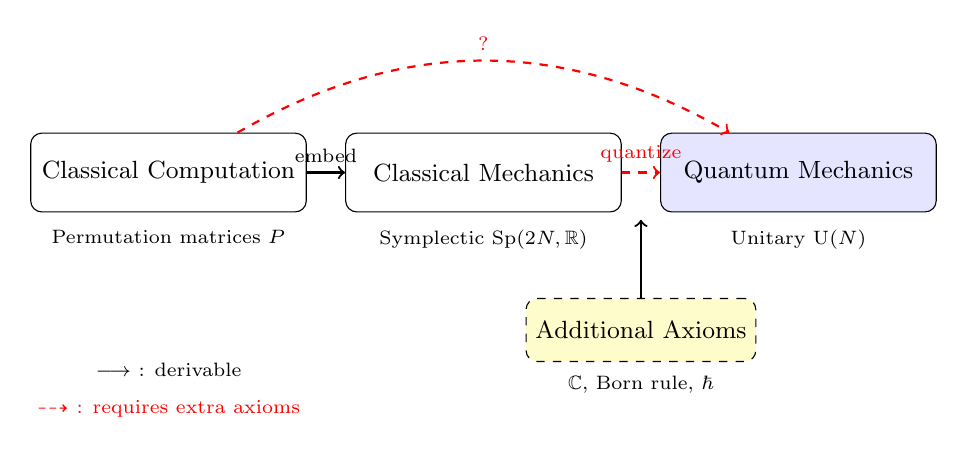
\begin{tikzpicture}[scale=1.0, every node/.style={font=\small}]
% Classical computation
\node[draw, rounded corners, minimum width=3.5cm, minimum height=1cm] (CC) at (-4, 0) {Classical Computation};
\node[below=0.1cm of CC, font=\scriptsize] {Permutation matrices $P$};

% Classical mechanics
\node[draw, rounded corners, minimum width=3.5cm, minimum height=1cm] (CM) at (0, 0) {Classical Mechanics};
\node[below=0.1cm of CM, font=\scriptsize] {Symplectic $\Sp(2N, \R)$};

% Quantum mechanics
\node[draw, rounded corners, minimum width=3.5cm, minimum height=1cm, fill=blue!10] (QM) at (4, 0) {Quantum Mechanics};
\node[below=0.1cm of QM, font=\scriptsize] {Unitary $\Un(N)$};

% Arrows
\draw[->, thick] (CC) -- (CM) node[midway, above, font=\scriptsize] {embed};
\draw[->, thick, dashed, red] (CM) -- (QM) node[midway, above, font=\scriptsize] {quantize};
\draw[->, thick, dashed, red] (CC) to[bend left=30] node[midway, above, font=\scriptsize] {?} (QM);

% Additional axioms box
\node[draw, dashed, rounded corners, minimum width=2.5cm, minimum height=0.8cm, fill=yellow!20] (AX) at (2, -2) {Additional Axioms};
\node[below=0.05cm of AX, font=\scriptsize] {$\C$, Born rule, $\hbar$};

\draw[->, thick] (AX) -- (2, -0.6);

% Legend
\node[font=\scriptsize] at (-4, -2.5) {$\longrightarrow$ : derivable};
\node[font=\scriptsize, red] at (-4, -3) {$\dashrightarrow$ : requires extra axioms};
\end{tikzpicture}
\end{center}

\textbf{Key insight}: The dashed arrows require external input:
\begin{enumerate}
    \item \textbf{Classical $\to$ Quantum} (standard quantization): Requires Planck's constant $\hbar$, the correspondence $\{q, p\} \to \frac{1}{i\hbar}[\hat{q}, \hat{p}]$, and the complex Hilbert space structure.
    \item \textbf{Computation $\to$ Quantum} (computational quantization): Requires all of the above, plus the Born rule to interpret amplitudes as probabilities.
\end{enumerate}

This diagram formalizes our main conclusion: no arrow from ``Classical Computation'' to ``Quantum Mechanics'' exists without passing through additional axioms.

\end{document}

